\chapter{Graphical User Interface}

\section{Motivation}
A \gls{gui} framework has been developed during the master thesis.
There were two main motivations behind this.

In order to operate a camera system in real time it is pretty usefull to be able to see what the camera sees.
During the \preproject a simple way of interacting with the system from a phone over \gls{ssh} through an app called juiceSSH was tested \cite[32]{martensPortableSensorRig2022}.
This app was tested more in the beginning of the master thesis, and several usefull snippets were saved in the app.
Although the text interface was sufficient to start and stop the recording and verify that images were saved, the lack of a graphical interface made it difficult to verify that the camera was recording what it was supposed to.
Thus a \gls{gui} is needed.

In a more general context a need for an efficient way to interact with programs and visualize data on remote computers was identified.
The \jx has been the current platform for the master thesis, but during future work other remote computers will be used.
A powerful workstation with a \todo was aquired last fall to be used for training and inference of \gls{ai} models during future Ph.D. work.
The workstation is headless, that is it has no monitor, keyboard or mouse, as we are a couple of people that will be using it.

\subsection{Specifications}
There are a lot of different options to choose from when it comes to \gls{gui} frameworks.
But the following requirements were identified:
\begin{itemize}
    \item Access from all devices including smartphone
    \item Easy to develop
    \item Capable of real time visualization
    \item Reasonably efficient
    \item Easily customizable
\end{itemize}
From the forst requirement it was clear that the solution would be web based as this it is the easiest way to make a \gls{gui} that is accessible from different types of devices.
Using a \gls{js} framework like React, Vue or Svelte would probably have been a good choice, but with very little personal experience using \gls{js} it appeared too ambitious to learn a new framework in a new language.
\dash was chosen as it is based on \py, making the learning curve less steep.


\dash is not designed for real time applications and lacks native support for \glsps{websocket}.
Fortunately a group of people have developed a package called \texttt{dash-extensions} that adds support for \glsps{websocket} to \dash \cite{eriksenDashExtensions}.
To improve performance the thread baced backend of \dash, Flask, was replaced with asynchronous Quart.

\subsection{Replacing Flask backend with Quart}

\subsection{Adding support for websockets}

\subsection{Websockets through Quart and Dash-Extentions}

\subsection{Custon JS handlers}

\subsection{Mantine}

\subsection{Video streaming}
Handling raw images is a pain in the ass but saves a lot of data compared to base64.

\subsection{ID Provider}
An aspect of working with \dash that can be slightly annoying is the use of id-strings.
The example below shows how the two id-strings \code{graph-content} and \code{dropdown-selection} are used when defining the components and when creating the callback.
\begin{listing}[H]
    \begin{minted}{python}
        app.layout = html.Div([
            html.H1(children='Title of Dash App', style={'textAlign':'center'}),
            dcc.Dropdown(df.country.unique(), 'Canada', id='dropdown-selection'),
            dcc.Graph(id='graph-content')
        ])

        @callback(
            Output('graph-content', 'figure'),
            Input('dropdown-selection', 'value')
        )
        def update_graph(value):
            dff = df[df.country==value]
            return px.line(dff, x='year', y='pop')
    \end{minted}
    \caption{Code showing the use of id string \cite{plotlyMinimalDashApp}}
\end{listing}

Modern \glspl{ide} like \gls{vscode} are capable of providing autocomplete suggestions, speeding up the code writing.
This works really well in for variable and property names, but not for strings.
For larger \dash projects name collisions can be a problem, and renaming a component through search and replace is not always straight forward.
To solve this annoyance a helper class called \code{IdProvider} was created.

Whenever a new attribute is accessed, like \code{IdProvider.variable1}, a new id-string is generated and returned as shown in Figure \ref{fig:idproider_a} and \ref{fig:idproider_c}.
When the program is finished, the \code{IdProvider.generate_code()} automatically generates the code for the \code{KnownIds} class, using \gls{jinja} templates with output as shown in Figure \ref{fig:idproider_b}.
The \code{KnownIds} is used for typing and have a property matching each of the attributes accesed through \code{IdProvider}.
As the \code{IdProvider} inherits from \code{KnownIds} this makes it possible to use autocomplete anv variable renaming on future calls to \code{IdProvider.variable1} as shown in \ref{fig:idproider_d}.
The \code{StrWithChilren} class is a subclass of \code{str} that makes it possible to add children to the id-string, such as \code{variable3.variable4} shown in Figure \ref{fig:idproider_b}.

\begin{figure}[H]
    \centering
    \subcaptionbox{Code on first run \label{fig:idproider_a}}{
        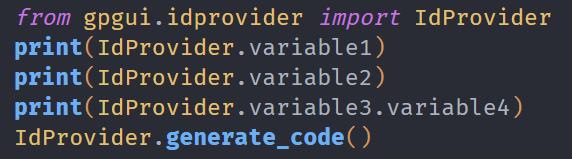
\includegraphics[width=0.6\textwidth]{figures/idp/idp1.png}

    }
    \subcaptionbox{Code on following runs, red color is from linter recognizing names \label{fig:idproider_b}}{
        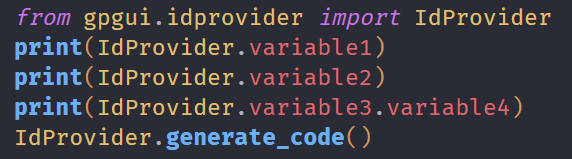
\includegraphics[width=0.6\textwidth]{figures/idp/idp2.png}
    }


    \subcaptionbox{Output from \textbf{(a)} or \textbf{(b) \label{fig:idproider_c}}}{
        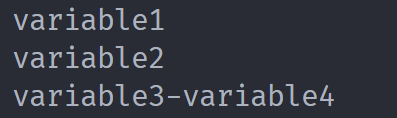
\includegraphics[width=0.4\textwidth]{figures/idp/idp4.png}
    }

    \subcaptionbox{Autogenerated after first run \label{fig:idproider_d}}{
        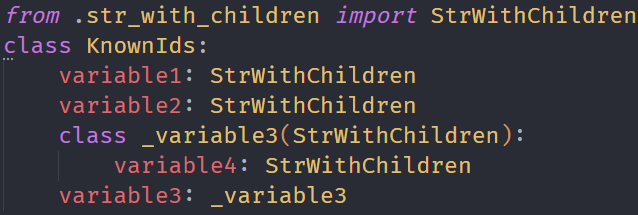
\includegraphics[width=0.6\textwidth]{figures/idp/idp3.png}

    }

    \caption{Visualization of the \code{IdProvider} class}
\end{figure}



